\subsection{Exercise~1.11}

By using universal properties, one always gets a continuous bijection from~$Y$ with the quotient topology to~$Y$ with the product topology.
This tells us that the quotient topology on~$Y$ is finer than the product topology.

However, these two topologies will typically not agree.



\subsubsection{General Remarks}

The author has no idea how the reader is supposed to come of with a counterexample on their own.
Searching for counterexample online reveals the following:
\begin{itemize}

	\item
		In \autocite[Exercise~I.§5.6, p.~128]{bourbaki_general_topoly_1} the following counterexample is given:
		\begin{quote}
			\itshape
			Let~$S$ be the equivalence relation on the rational line~$\mathbf{Q}$ which is obtained by identifying all the points of~$\mathbf{Z}$.
			Show that~$S$ is closed, and that if~\,$U$\! is the relation of equality on~$\mathbf{Q}$, then the canonical bijection of~$(\mathbf{Q} × \mathbf{Q}) / (U × S)$ onto~$\mathbf{Q} × (\mathbf{Q} / S)$ is not a homeomorphism.
		\end{quote}
		Although according to \autocite{freedom_math_dance_quotient_product_bourbaki}, an earlier (French) versions of the book still erroneously claimed that the product topology is compatible with the quotient topology.

	\item
		This counterexample is also given in \cite[4.3, Example, p.~111]{brown_topology_and_groupoids}:
		\begin{quote}
			\itshape
			We now show that 4.3.2 is false without some assumptions on~$B$.
			Let~$f \colon ℚ \to ℚ / ℤ$ be the identification map and let
			\[
				h = f × 1 \colon ℚ × ℚ \to (ℚ / ℤ) × ℚ \,.
			\]
			Then~$h$ is not an identification map.
		\end{quote}

	\item
		The same counterexample can also be found in \autocite[Chapter~2, §22, Example~7, p.~141]{munkres_topology}:
		\begin{quote}
			\itshape
			Let~$X = ℝ$ and let~$X^*$ be the quotient space obtained from~$X$ by identifying the subset~$ℤ_+$ to a point~$b$;
			let~$p \colon X \to X^*$ be the quotient map.
			Let~$ℚ$ be the subspace of~\,$ℝ$ consisting of the rational numbers;
			let~$i \colon ℚ \to ℚ$ be the identity map.
			We show that
			\[
				p × i \colon X × ℚ \to X^* × ℚ
			\]
			is not a quotient map.
		\end{quote}

	\item
		Another counterexample in the same vein is given in \autocite{stackexchange_relation_product_quotient_topology}, based on \autocite[Exercise~4.4.7]{boekstedt_vosegaard_point_set_topology}:
		\begin{quote}
			\itshape
			Let~$ℚ_{> 0}$ denote the positive rational numbers.
			Let~$∼_1$ be the equivalence relation on the numbers generated by the requirement~$x ∼_1 y$ if both~$x$ and~$y$ are integers.
			Let~$ℚ_{> 0} / {∼_1}$ be the quotient space, with quotient map~$π_1 \colon ℚ_{> 0} \to ℚ_{> 0} / {∼_1}$.
			In the same way, we consider the equivalence relation~$∼_2$ on~$ℚ_{> 0} × ℚ$, generated by requiring that~$(x, y) ∼_2 (u, y)$ if both~$x$ and~$u$ are integers.
			Denote the corresponding quotient map by~$π_2 \colon ℚ_{> 0} × ℚ \to (ℚ_{> 0} × ℚ) / {∼_2}$.
			\begin{enumerate}[label=\arabic*.]

				\item
					Show that there is a unique map (of sets)
					\[
						f \colon (ℚ_{> 0} × ℚ) / {∼_2} \to ℚ_{> 0} / {∼_1} × ℚ
					\]
					with the property that~$f(π_2(x, y)) = (π_1(x), y)$.
					Show that~$f$ defined a continuous, bijective map.

				\item
					For each natural number~$n ≥ 1$, we define
					\[
						U_n
						=
						\biggl\{
							(x, y) ∈ ℚ_{> 0} × ℚ
							\suchthat[\bigg]
							\abs{x - n}
							<
							\min\biggl\{ \abs[\bigg]{ y - \frac{\sqrt{2}}{n} }, \frac{1}{2} \biggr\}
						\biggr\} \,,
					\]
					and we put
					\[
						U = ⋃_{n ≥ 1} U_n \,.
					\]
					Show that~$π_2(U)$ is open.
					(Hint: Use that~$\sqrt{2}$ is irrational to prove that~$π_2^{-1} π_2(U) = U$.)
				\item
					Let~$ε > 0$ and~$n ∈ ℕ$.
					Assume that~$\sqrt{2} / n < ε$.
					Prove that there are no~$a < n < b$ so that
					\[
						\{
							(x, y) ∈ ℚ_{> 0} × ℚ
							\suchthat
							\text{$a < x < b$ and~$-ε < y < ε$}
						\}
						\subset
						U_n \,.
					\]

				\item
					Show that the set~$f(π_2(U))$ is not a neighbourhood of the element $(π_1(1), 0)$.
					In particular, the set is not open.

				\item
					Conclude that~$f$ is not a homeomorphism.

			\end{enumerate}
		\end{quote}

	\item
		In \autocite[Chapter~2, §22, Exercise~6, p.~143]{munkres_topology} a related example is given:
		\begin{quote}
			\itshape
			Recall that~$ℝ_K$ denotes the real line with the~\topology{$K$}.
			(See~§13.)
			Let~$Y$ be the quotient space obtained from~$ℝ_K$ by collapsing the set~$K$ to a point;
			let~$p \colon ℝ_K \to Y$ be the quotient map.
			\begin{enumerate}[label=(\alph*\upshape)]

				\item
					Show that~$Y$ satisfies the $T_1$ axiom, but is not Hausdorff.

				\item
					Show that~$p × p \colon ℝ_K × ℝ_K \to Y × Y$ is not a quotient map.
					\textup[\emph{Hint}:
					The diagonal is not closed in~$Y × Y$, but its inverse image is closed in~$ℝ_K × ℝ_K$.\textup]

			\end{enumerate}
		\end{quote}
		The~\topology{$K$} mentioned here is defined as follows:
		the set~$K$ is defined as~$\{ 1/n \suchthat n ∈ ℤ_+ \}$, and the~\topology{$K$} on~$ℝ$ is generated by all open intervals~$(a, b)$ together with all sets of the form~$(a, b) ∖ K$.
		(The~\topology{$K$} is thus finer than the standard topology.)


	\item
		A different kind of counterexample is given in \cite{fabel_hawaiian_earring_discontinuous}:
		\begin{quote}
			\itshape
			If~$L(X, p)$ denotes the space of~$p$ based loops in~$X$ with the compact open topology, and if~$q \colon L(X, p) \to π_1(X, p)$ is the natural surjection, endow~$π_1(X, p)$ with the quotient topology \textup[…\textup].

			The \textbf{Hawaiian earring}~$HE$ is the union of a null sequence of circles joined at a common point~$p$.
			Formally,~$HE$ is the following subspace of the plane~$R^2$, for an integer~$n ≥ 1$ let~$X_n$ denote the circle of radius~$1/n$ centered at~$(1/n, 0)$ and define~$HE = ⋃_{n = 1}^∞ X_n$.
			Let~$p = (0, 0)$ \textup[…\textup].

			\textbf{Theorem 1.}
			The product of quotient maps
			\[
				q × q \colon L(HE, p) × L(HE, p) \to π_1(HE, p) × π_p(HE, p)
			\]
			fails to be a quotient map \textup[…\textup].
		\end{quote}

	\item
		A vast generalization of the above counterexample can apparently be found in \cite{brazas_topological_fundamental_group}.
\end{itemize}



\subsubsection{A Specific Counterexample}

Let~$∼$ be the equivalence relation on~$ℝ$ that identifies all integers, and leaves all other numbers unidentified.
Let~$S ≔ ℝ / {∼}$ and let~$π$ be the quotient map from~$ℝ$ to~$S$.
We denote the set~$S × ℚ$ together with the product topology by~$P$, and together with the quotient topology by~$Q$.
We denote the induced equivalence relation on~$ℝ × ℚ$ again by~$∼$;
it identifies for every rational number~$y$ all points of the form~$(n, y)$ with~$n ∈ ℤ$.

We know from \nameref{exercise 1.9} that the product topology on~$ℝ × ℚ$ agrees with the subspace topology coming from~$ℝ^2$.
We will therefore regard the product~$ℝ × ℚ$ as a subspace of~$ℝ^2$.

For every integer~$n$ let~$r_n ≔ \sqrt{2} / (\abs{n} + 1)$.
These are irrational numbers with~$r_n \to 0$ as~$n \to ∞$.
For every integer~$n$ let~$T'_n$ be the closed triangle in~$ℝ^2$ with endpoints
\[
	(n, r_n) \,, \quad
	\Bigl(n + \frac{1}{4}, r_n + \frac{1}{4}\Bigr) \,, \quad
	\Bigl(n + \frac{1}{4}, r_n - \frac{1}{4}\Bigr) \,.
\]
This set may also be described as
\[
	T'_n
	≔
	\{
		(x, y) ∈ ℝ^2
		\suchthat
		\text{$x ∈ [n, n + 1/4]$ and~$\abs{y - r_n} ≤ x - n$}
	\} \,.
\]
In terms of pictures,~$T'_n$ is a triangle pointing towards the point~$(n, r_n)$, see \cref{image of the triangle set}.
\begin{figure}
	\centering
	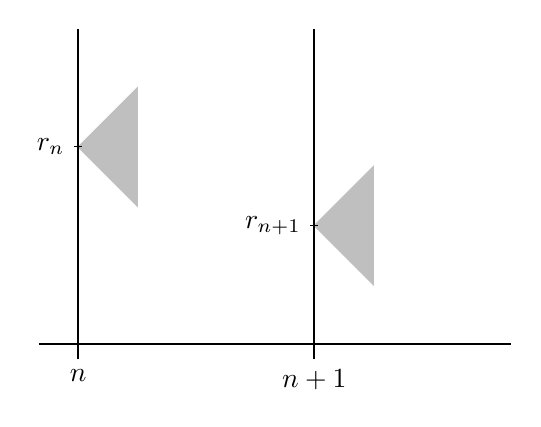
\begin{tikzpicture}
		% horizontal line
		\draw[thick] (-0.5, 0) -- (5.5, 0);
		% the triangle
		\draw[fill, gray!50] (0, 2.5) -- ++(0.75, 0.75) -- ++(0, -1.5) -- cycle;
		\draw[fill, gray!50] (3, 1.5) -- ++(0.75, 0.75) -- ++(0, -1.5) -- cycle;
		% vertical lines
		\draw[thick] (0, -0.2) node[below] {$n$} -- (0, 4);
		\draw[thick] (3, -0.2) node[below] {$n + 1$} -- (3, 4);
		% the points (n, r_n) and (n+1, r_{n+1})
		\draw (-0.05, 2.5) node[left] {$r_n$} -- ++(0.1, 0);
		\draw (2.95, 1.5) node[left] {$r_{n + 1}$} -- ++(0.1, 0);
	\end{tikzpicture}
	\caption{The sets~$T'_n$ and~$T'_{n + 1}$.}
	\label{image of the triangle set}
\end{figure}
We set~$T_n ≔ T'_n ∩ (ℝ × ℚ)$.
Here is the important part:

The corner point~$(n, r_n)$ of the triangle~$T'_n$ is not contained in~$T_n$ because~$\sqrt{2}$ is irrational, but it can still be approximated by points of~$T_n$.
In fact, the set~$T_n$ is entirely contained in~$(n, n + 1) × ℚ$, and is therefore saturated with respect to the equivalence relation~$∼$ on~$ℝ × ℚ$.
Also, since the triangle~$T'_n$ is closed in~$ℝ^2$, the set~$T_n$ is closed in~$ℝ × ℚ$.

We note that the set~$T' ≔ ⋃_{n ∈ ℤ} T'_n$ is again closed in~$ℝ^2$.
It follows that
\[
	T ≔ ⋃_{n ∈ ℤ} T_n = ⋃_{n ∈ ℤ} T'_n ∩ (ℝ × ℚ)
\]
is again closed in~$ℝ × ℚ$.
The set~$T$ is also saturated because each~$T_n$ is saturated.

Let~$T_Q$ be the image of~$T$ in~$Q$.
This set is closed in~$Q$ because~$T$ is both closed and saturated in~$ℝ × ℚ$.

Let similarly~$T_P$ be the image of~$T$ in~$P$.
We claim that the set~$T_P$ is \emph{not} closed in~$P$.
Suppose otherwise.
The complement of~$T_P$ is then open, and it contains the point~$(\class{0}, 0)$.
There hence exist open subsets~$W$ and~$V$ of~$S$ and~$ℚ$ respectively such that
\[
	(\class{0}, 0) ∈ W × V ⊆ P ∖ T_P \,.
\]
Let~$U$ be the preimage of~$W$ in~$ℝ$;
this is an open subset of~$ℝ$ with
\[
	ℤ × \{ 0 \} ⊆ U × V ⊆ (ℝ × ℚ) ∖ T \,.
\]
The set~$V$ is an open neighbourhood of~$0$ in~$ℚ$, so there exists some~$ε > 0$ with~$(-ε, ε)_ℚ ⊆ V$.
We then have
\[
	ℤ × \{ 0 \} ⊆ U × (-ε, ε)_ℚ ⊆ (ℝ × ℚ) ∖ T \,.
\]
This tells us that the two sets~$U × (-ε, ε)_ℚ$ and~$T$ are disjoint.
But this cannot be:
let~$n$ be sufficiently large such that~$r_n < ε$.
The point~$x ≔ (n, r_n)$ in~$ℝ^2$ is then contained in~$U × (-ε, ε)_ℝ$;
see \cref{triangle intersects neighbourhood}.
\begin{figure}
	\centering
	\begin{tikzpicture}
		% horizontal line
		\draw[thick] (-2.5, 0) -- (2.5, 0);
		% vertical line
		\draw[thick] (0, -0.2) node[below]{$n$} -- (0, 5);
		% the triangle
		\draw[fill, gray!50] (0, 2.5) -- ++(2, 2) -- ++(0, -4) -- cycle;
		% point (n, r_n)
		\draw (-0.1, 2.5) node[left]{$r_n$} -- (0.1, 2.5);
		% open set
		\draw[dashed] (-1, -0.2) -- (-1, 4) node[below left]{\begin{tabular}{l}$U × (-ε, ε)_ℝ$ \\ around~$n$\end{tabular}} -- (1, 4) -- (1, -0.2);
	\end{tikzpicture}
	\caption{Once~$r_n$ is small enough, the point~$(n, r_n)$ is contained in~$U × (-ε, ε)_ℝ$, which is then intersected by~$T'_n$.}
	\label{triangle intersects neighbourhood}
\end{figure}
This means that inside~$ℝ^2$, the set~$U × (-ε, ε)_ℝ$ is an open neighbourhood of~$x$.
While the point~$x$ is not contained in the triangle~$T_n ⊆ ℝ × ℚ$, it can still be approximated by points in this triangle.
There hence exists a point~$y$ in~$T_n$ that is contained in the specific neighbourhood~$U × (-ε, ε)_ℝ$ of~$x$.
Since~$y ∈ T_n ⊆ ℝ × ℚ$, we already have~$y ∈ (U × (-ε, ε)_ℝ) ∩ (ℝ × ℚ) = U × (-ε, ε)_ℚ$.
Therefore,~$y$ is a point in both~$T_n$ and~$U × (-ε, ε)_ℚ$, contradicting the disjointness of~$T$ and~$U × (-ε, ε)_ℚ$.
